\documentclass{article}
\usepackage{amssymb}
\usepackage{microtype}
\usepackage{tikz}

\title{Modes of Convergence}
\author{William G Underwood}

\begin{document}

\maketitle

\section{Introduction}

In probability theory, we use several notions of `convergence' for
a sequence of random variables.
Some of these notions are stronger than others, so it is natural to ask
exactly when one convergence implies another.
In the following definitions and results, we assume that $X$ and $(X_n)_{n \geq 1}$ are all
random variables on some probability space.







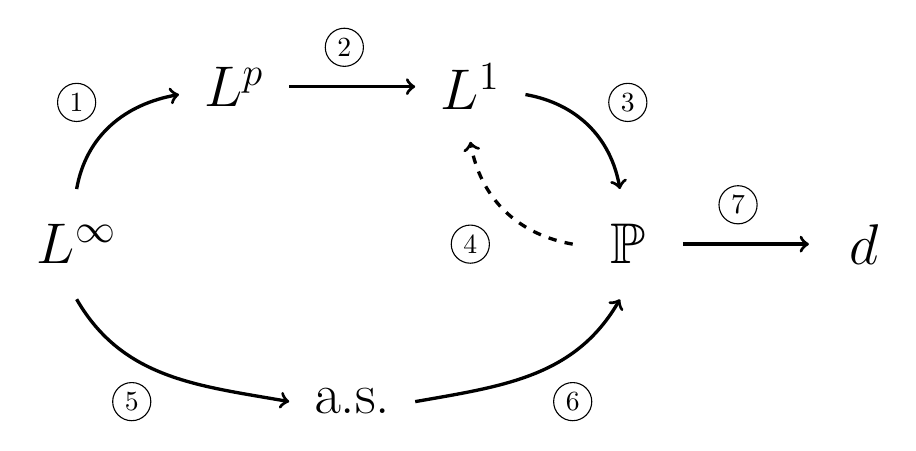
\begin{tikzpicture}

  % nodes
  \node at (0,0) {\huge $L^\infty$};
  \node at (2,2) {\huge $L^p$};
  \node at (5,2) {\huge $L^1$};
  \node at (7,0) {\huge $\mathbb{P}$};
  \node at (10,0) {\huge $d$};
  \node at (3.5,-2) {\huge a.s.};

  % arrows
  \draw [->, very thick] (0,0.7) to [out=80,in=190] (1.3,1.9);
  \draw [->, very thick] (2.7,2) -- (4.3,2);
  \draw [->, very thick] (5.7,1.9) to [out=-10,in=100] (6.9,0.7);
  \draw [->, very thick, dashed] (6.3,0) to [out=170,in=-80] (5,1.3);
  \draw [->, very thick] (7.7,0) -- (9.3,0);
  \draw [->, very thick] (0,-0.7) to [out=-60,in=170] (2.7,-2);
  \draw [->, very thick] (4.3,-2) to [out=10,in=-120] (6.9,-0.7);

  % labels
  \node[circle,draw,inner sep=2pt] at (0,1.8) {1};
  \node[circle,draw,inner sep=2pt] at (3.4,2.5) {2};
  \node[circle,draw,inner sep=2pt] at (7,1.8) {3};
  \node[circle,draw,inner sep=2pt] at (5,0) {4};
  \node[circle,draw,inner sep=2pt] at (0.7,-2) {5};
  \node[circle,draw,inner sep=2pt] at (6.3,-2) {6};
  \node[circle,draw,inner sep=2pt] at (8.4,0.5) {7};

\end{tikzpicture}

\end{document}
